%File: formatting-instruction.tex
\documentclass[letterpaper]{article}
\usepackage{aaai}
\usepackage{times}
\usepackage{helvet}
\usepackage{courier}
\usepackage{graphicx}
\usepackage{amssymb}
\usepackage{algorithm}
% \usepackage[]{algorithm2e}
% \usepackage[]{algorithmic}
\usepackage{algpseudocode}
% \usepackage{algorithm}
\usepackage{mathtools}

\frenchspacing
\setlength{\pdfpagewidth}{8.5in}
\setlength{\pdfpageheight}{11in}
\pdfinfo{
/Title (Voice Conversion using GANs)
/Author (Varun Sreedhara Bhatt, Arka Sadhu, Karan Taneja)}
\setcounter{secnumdepth}{0}  
 \begin{document}
\title{Voice Conversion using Generative Adversarial Networks}
\author{Varun Sreedhara Bhatt \\
140260004
\And
Arka Sadhu \\
140070011
\And
Karan Taneja \\
15D070022
}
\nocopyright
\maketitle
\begin{abstract}
\begin{quote}
Voice conversion is the task of converting speech of a source speaker as a target speaker would have said it. This project considers the case of non-parallel dataset where the source and target speakers don't speak the same sentence in the training set and shows that using sentence embeddings in combination with WGAN can give an improvement over existing methods.
\end{quote}
\end{abstract}

\section{Task Definition}
We are given an audio input from speaker $s$ from which we obtain the spectral frames $X_s=\{x_{s,n}\}_{n=1}^{N_s}$ where $N_s$ is the number of spectral frames. We are also given a target speaker $t$ for which we have to generate spectral frames $X_t=\{x_{t,n}\}_{n=1}^{N_t}$ and therefore the audio output. The audio output should be such that it sounds like target speaker $t$ speaking the linguistic content of $X_s$. The most common way to evaluate voice conversion systems currently is to get subjective opinion from listeners. This is quantified using the metric called Mean Opinion Score (MOS). Metrics like mean cepstral coefficients are not used as the findings from this metric is not consistent with human evaluation \cite{vawgan}.

The work is done using the dataset provided by Voice Conversion Challenge 2018 \footnote{http://vc-challenge.org/}. In this task, in addition to the source and target voice samples in both parallel and non-parallel settings, we are also given the corresponding transcriptions. All voice samples are in English and so are the transcriptions. In this work we extend earlier concepts on similar data (Voice Conversion Challenge 2016) to exploit this extra information provided by the transcriptions.

\section{Methodology}
There are two ways in which voice conversion can be done, namely parallel and non-parallel. In parallel voice conversion, both source and target speaker say the same text while in non-parallel, the text spoken can be different. 

Broadly, the idea in voice conversion is to separate a speech into speaker independent and speaker dependent encoding. The speaker independent part is then combined with the speaker characteristics of the target speaker to generate the speech as spoken by the target speaker. In parallel case, the speaker independent part will be same for both source speech and target speech during training which can be used to better separate the speaker dependent part. 

\subsection{C-VAE}
The task here is non-parallel as is given in \cite{vae}. A conditional Variational Autoencoder (c-VAE) \cite{NIPS2015_5775} is used to encode ($\mathcal{E}$) the source speech ($X_s$) into a speaker independent representation ($z$). It is then concatenated with the one-hot vector of the target speaker ($y$) and passed through a decoder (generator, $\mathcal{G}$) to get the target speech ($X_t$) as given in ~\cite{vae}.

During training, encoder minimizes the KL-divergence between $z$ and standard normal distribution $\mathcal{N}(0,1)$. The encoder and decoder together maximize the log likelihood of data $\log p(X|z,y)=\mathcal{N}(\mathcal{G}(z,y),I)$. The overall cost to minimize then becomes
\[J_{vae}=\mathcal{D}_{KL}(z||\mathcal{N}(0,1)) - \log p(X|z,y) \]

Since $z$ is a sample from a distribution which depends on the encoder, it is not possible to do back-propagation through it. Hence, it is re-parametrized as $\mathcal{N}(\mathcal{E_\mu}(X), diag(\mathcal{E_\sigma}(X))$. $z$ can then be written as $\mathcal{E_\mu}(X)+diag(\mathcal{E_\sigma}(X))\epsilon$ where $\epsilon$ is a sample of $\mathcal{N}(0,I)$. Figure \ref{fig:vae} shows the architecture of c-VAE.

\begin{figure}[h]
	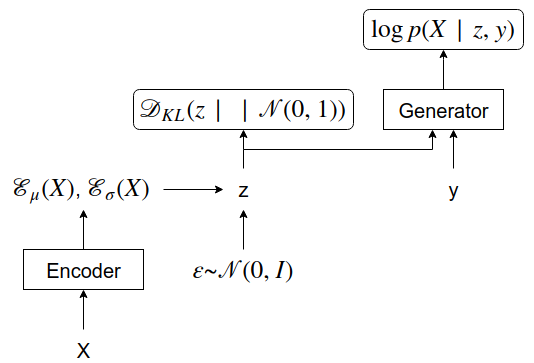
\includegraphics[width=8cm]{images/VAE_network}
    \caption{Architecture of c-VAE}
	\label{fig:vae}
\end{figure}

\subsection{VAWGAN}
\cite{vawgan} extend this idea further by adding a Wasserstein objective function to the generator. A discriminator network is added to the system which finds the Wasserstein distance between the input and the generated speech. The generator tries to minimize this distance while also maximizing the log likelihood.

\cite{wgan} define Wasserstein distance between 2 probability distributions $\mathbb{P}_r$ and $\mathbb{P}_g$ as
\[W(\mathbb{P}_r, \mathbb{P}_g)=\inf_{\gamma \in \Pi(\mathbb{P}_r,\mathbb{P}_g)} \mathbb{E}_{(x,y)\sim \gamma} \left[||x-y|| \right] \]
Here, $\Pi(\mathbb{P}_r,\mathbb{P}_g)$ is the set of all joint distributions whose marginals are $\mathbb{P}_r$ and $\mathbb{P}_g$. This distance is also called as Earth Mover distance since this is the amount of probability mass that needs to be moved to convert $\mathbb{P}_r$ into $\mathbb{P}_g$ (or vice versa).

Calculating the infimum is computationally intractable and hence the above distance is approximated as
\[W(\mathbb{P}_r, \mathbb{P}_g)=\sup_{||f||_L \leq 1} \mathbb{E}_{x\sim \mathbb{P}_r} \left[f(x)\right] - \mathbb{E}_{x\sim \mathbb{P}_g} \left[f(x)\right] \]
$||f||_L \leq 1$ denotes all 1-Lipschitz functions.

The discriminator network parametrizes 1-Lipschitz functions $f$ (either by clipping the weights or by introducing a gradient penalty). $\mathbb{P}_r$ is the distribution corresponding to data and $\mathbb{P}_g$ is the distribution corresponding to the generated data. Every data point given during training is a sample from the data distribution. The output generated after passing it through encoder and generator is a sample from the generated data distribution. Passing them through discriminator gives $f(x)$ and $f(x_g)$ where x is the original data and $x_g$ is the generated data. Thus, the loss function for the discriminator network is given by
\[J_{wgan}= f(X)-f(X|z,y) \]

The discriminator needs to maximize this loss while generator needs to minimize it. When combined with the c-VAE architecture, the total loss function for the generator to minimize becomes 
\[J_{gen}=-\log p(X|z,y) + \alpha J_{wgan} \]
where $\alpha$ is a parameter controlling the contribution of Wasserstein distance to the loss. Figure \ref{fig:vawgan} shows the architecture of the system with WGAN added.

\begin{figure}[h]
	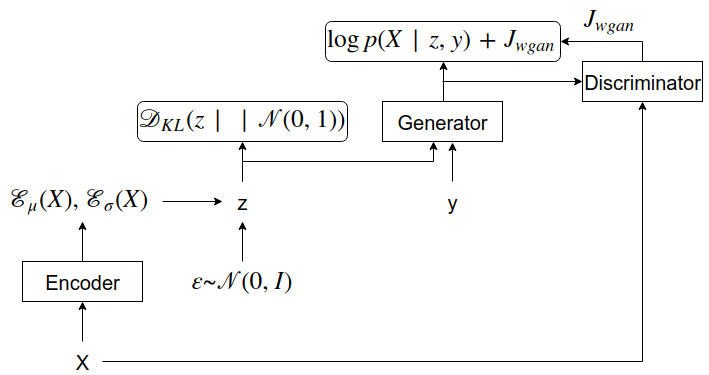
\includegraphics[width=8cm]{images/VAWGAN_network}
    \caption{Architecture of VAWGAN}
	\label{fig:vawgan}
\end{figure}

\subsection{VAWGAN-S}
In this work we extend this idea further to incorporate sentence embeddings of the sentence spoken as well. In the Voice Conversion Challenge 2018, %Need to cite the challenge explicitly%
the training data also contains transcriptions which is used during training. The architecture proposed is shown in figure \ref{fig:vawgans}.

\begin{figure}
	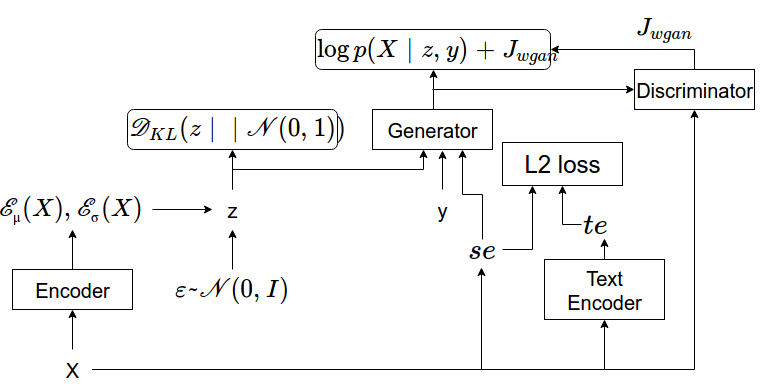
\includegraphics[width=8cm]{images/VAWGAN_S}
    \caption{Architecture of VAWGAN-S}
    \label{fig:vawgans}
\end{figure}

We first get a good representation for the sentence by following the algorithm given in \cite{arora2017asimple}.
%A brief description is given here. Theoretical justification and experimental details can be found in the paper.
The algorithm assumes that we have some word embeddings. For this task we use the word embeddings provided by fasttext \footnote{https://github.com/facebookresearch/fastText} \cite{bojanowski2016enriching} which gives a 300-dimensional vector for each word. Now given a set of sentences we directly get a weighted mean of word vectors forming the sentence. The weight is given by $\frac{a}{a + p(w)}$ with $a$ being a hyper-parameter and $p(w)$ being the unigram probability. Sentence vector is therefore calculate as below
\[v_s \leftarrow \frac{1}{|s|}\sum_{w\in s}\frac{a}{a+p(w)}v_w\] 
This gives us a vector $v_s$ for each sentence. This is followed by getting the first singular value of the matrix formed by $v_s$ as its columns which we call $u$. For each $v_s$ its projection on this vector is subtracted out to get the embedded sentence vector
\[v_s \leftarrow v_s - u u^T v_s\]

We note that at test time there is no transcription given, so ideally we would like an encoder which produces the sentence embeddings. For this purpose we add another encoder called the text encoder which given speech data extracts out the sentence embeddings. 

We had initially thought of using an explicit ASR system which could output an actual text which could further be embedded using the above algorithm but we didn't pursue this line of thought as this method would ultimately be limited by the efficiency of ASR system because if the word can't be decoded, it cannot be henceforth embedded. Instead of this, we use the text encoder which would find the function directly from the speech features space to the sentence embedding space.

Once we have the sentence embeddings we pass it to the generator which makes use of the vector obtained from previous encoding as well as the speaker id which is encoded as a one-hot vector to generate the output. The rest of the discriminator part remains the same as that in the VAWGAN. 
\begin{algorithm} % enter the algorithm environment
\caption{Algorithm to train VAWGAN-S} % give the algorithm a caption
\label{alg1} % and a label for \ref{} commands later in the document
\begin{algorithmic} % enter the algorithmic environment
    \Function {AutoEncode}{$X, y, t$}:
    	\State $Z_{\mu} \leftarrow \mathcal{E_{\phi_{E}}}_1(X)$
        \State $Z_{\sigma} \leftarrow \mathcal{E_{\phi_{E}}}_2(X)$
        \State $Z \leftarrow $ sample from $\mathcal{N}(Z_\mu, Z_\sigma)$
        \State $T \leftarrow \mathcal{E_{\phi_T}}(X)$
        \State $X' \leftarrow \mathcal(G)_{\theta}(Z_s, y, T)$
        \State \Return $X', Z, T$
    \EndFunction
    \State Initialize $\phi_E$, $\phi_T$, $\theta$, $\psi$
    \While{not converged do}
	\State $X_s, T_s \leftarrow$ minibatch of samples from source
    \State $X_t, T_t \leftarrow$ minibatch of samples from target
    \State $X_s', Z_s, T_s' \leftarrow AutoEncode(X_s, y_s, T_s)$
    \State $X_t', Z_t, T_t' \leftarrow AutoEncode(X_t, y_t, T_t)$
    \State $X_t|s \leftarrow \mathcal{G_\theta}(Z_s, T_s, y_t)$
	\State $J_{obs} \leftarrow J_{obs}(X_s) + J_{obs}(X_t)$
    \State $J_{lat} \leftarrow J_{lat}(Z_s) + J_{lat}(Z_t)$
    \State $J_{wgan} \leftarrow J_{wgan}(X_t, X_s)$
    \State $J_{tl} \leftarrow J_{tl}(T_s,T_s')$
    \While{not converged do}
    \State $\psi \xleftarrow{update} - \nabla_{\psi}(-J_{wgan})$
    \State $\phi_E \xleftarrow{update} - \nabla_{\phi_E}(J_{obs} + J_{lat})$
    \State $\phi_T \xleftarrow{update} -\nabla_{\phi_T}(J_{tl})$
    \State $\theta \xleftarrow{update} -\nabla_{\theta}(J_{obs} + \alpha J_{wgan})$
    \EndWhile
    \EndWhile
\end{algorithmic}
\end{algorithm}
\section{Implementation Details}
\subsection{VAWGAN}
We started with the code give by \cite{vae} for voice conversion using VAE \footnote{https://github.com/JeremyCCHsu/vae-npvc}. Speech is first converted into spectral features using pyworld vocoder. The spectral features are then passed into a CNN which acts as the encoder. The output of this CNN is concatenated with the one-hot representation of the speaker and passed into another CNN which acts as the generator. 

We then added the discrminator network to it. The generated output and the original data are passed through the discriminator to get the Wasserstein distance. The networks are then trained using their corresponding losses. The hyperparameter values and the network architectures were same as that given in \cite{vawgan}.
% <brief description of network parameters (kernel/strides) used for vawgan> or give reference
% <1 paragraph about training and hyper parameter setting>
% <citations required for hyper parameters taken from> 
% <Add a few details about training time it required for w-dist to start decreasing, alternatively it might also go into results and discussion>
\subsection{VAWGAN-S}
The implementation of VAE and WGAN part is kept the same as detailed above. To get the sentence embedding we use pre-trained vectors from FastText \cite{bojanowski2016enriching}. To get the unigram probability distribution we initially used the corpus WikiText2 \cite{DBLP:journals/corr/MerityXBS16}. Unfortunately, this corpus doesn't include common words used in spoken English. For eg., the corpus didn't include the word "I" which is expected because of the form of sentences used in the corpus. We then considered using the corpus provided by Peter Norvig \footnote{http://norvig.com/ngrams/} which uses $\frac{1}{3}$ million most frequent words to generate the unigram distribution. We expect similar sentence embedding because as it is mentioned in \cite{arora2017asimple} that the embeddings generalizes across different corpus. There is a hyperparameter $a$ used in weighing different words which we set it as a constant $10^{-3}$ which is the same as used in the paper. 

Now we train a text encoder to generate this sentence embeddings. The structure of the text encoder is exactly the same as that of the encoder used in VAWGAN (explained above). For training, since we have the transcriptions, we directly give the sentence embeddings to the generator, and use a l2-loss metric for the output of the text encoder and the sentence embedding as is shown in \ref{fig:vawgans}. It is noted that the l2 loss saturates very quickly. 

At test time, we get two encodings $z$ and $t_{enc}$. The generator now makes use of this new $t_{enc}$ to generate the audio output. 

% Algorithm for the complete system including sentence embedding

\section{Experimental Setup}

Voice conversion challenge 2018 dataset \footnote{http://vc-challenge.org/} is used for experimentation. The challenge has two tasks HUB and SPOKE tasks. HUB task consists of parallel training data while the SPOKE task has non-parallel data. For the HUB task, there are 4 source speakers and 4 target speakers (2 males and 2 females in each). Each speaker utters the same set of 81 sentences. For the SPOKE task there are 4 other source speaker (again 2 males and 2 females) and the target speakers remain the same as from the HUB task.The dataset also provides the corresponding text transcriptions for each HUB and SPOKE task. 

The evaluation metric we choose is Mean Opinion Score (MOS), i.e. subjective scores made by different people as is the standard in the literature for voice conversion \cite{vawgan}. The rating is on a scale of 1-5, with 1 being poor and 5 being excellent. We gave the users voice samples of the source, actual target, voice converted VAE baseline and voice converted using VAWGAN. The information about the last two is hidden from the user. The user is additionally asked about the gender identification of the output voice. We give a total of four samples one from each Female to Female, Male to Male, Female to Male, Male to Female.

\section{Results and Discussions}

Overall VAWGAN ratings are better than VAE baseline which is consistent with the results presented in \cite{vawgan}. VAWGAN clearly outperforms VAE baseline model in both inter-gender and intra-gender conversion tasks as seen in figures \ref{fig:mos} and \ref{fig:comparison}. MOS is higher in both cases and even in a direct comparison, speech from VAWGAN is regarded better. Decrease in MOS for both the architectures between intra-gender and inter-gender shows that inter-gender conversion in general more difficult than intra-gender. 
 
Gender identification errors (errors in identifying the gender of the target speaker) in inter-gender conversion in higher VAE baseline model compared to VAWGAN. This shows that the addition of Wasserstein objective function led the generator to better combine the encoded information and speaker characteristics.

The length of the sentence played a role in the quality of conversion. VCC 2018 dataset has much longer sentences as compared to VCC 2016 dataset and it directly affects conversion, decreasing the MOS. We believe that allowing variable size feature length (by using a sequential architecture) could solve this problem.

\begin{figure}[h]
	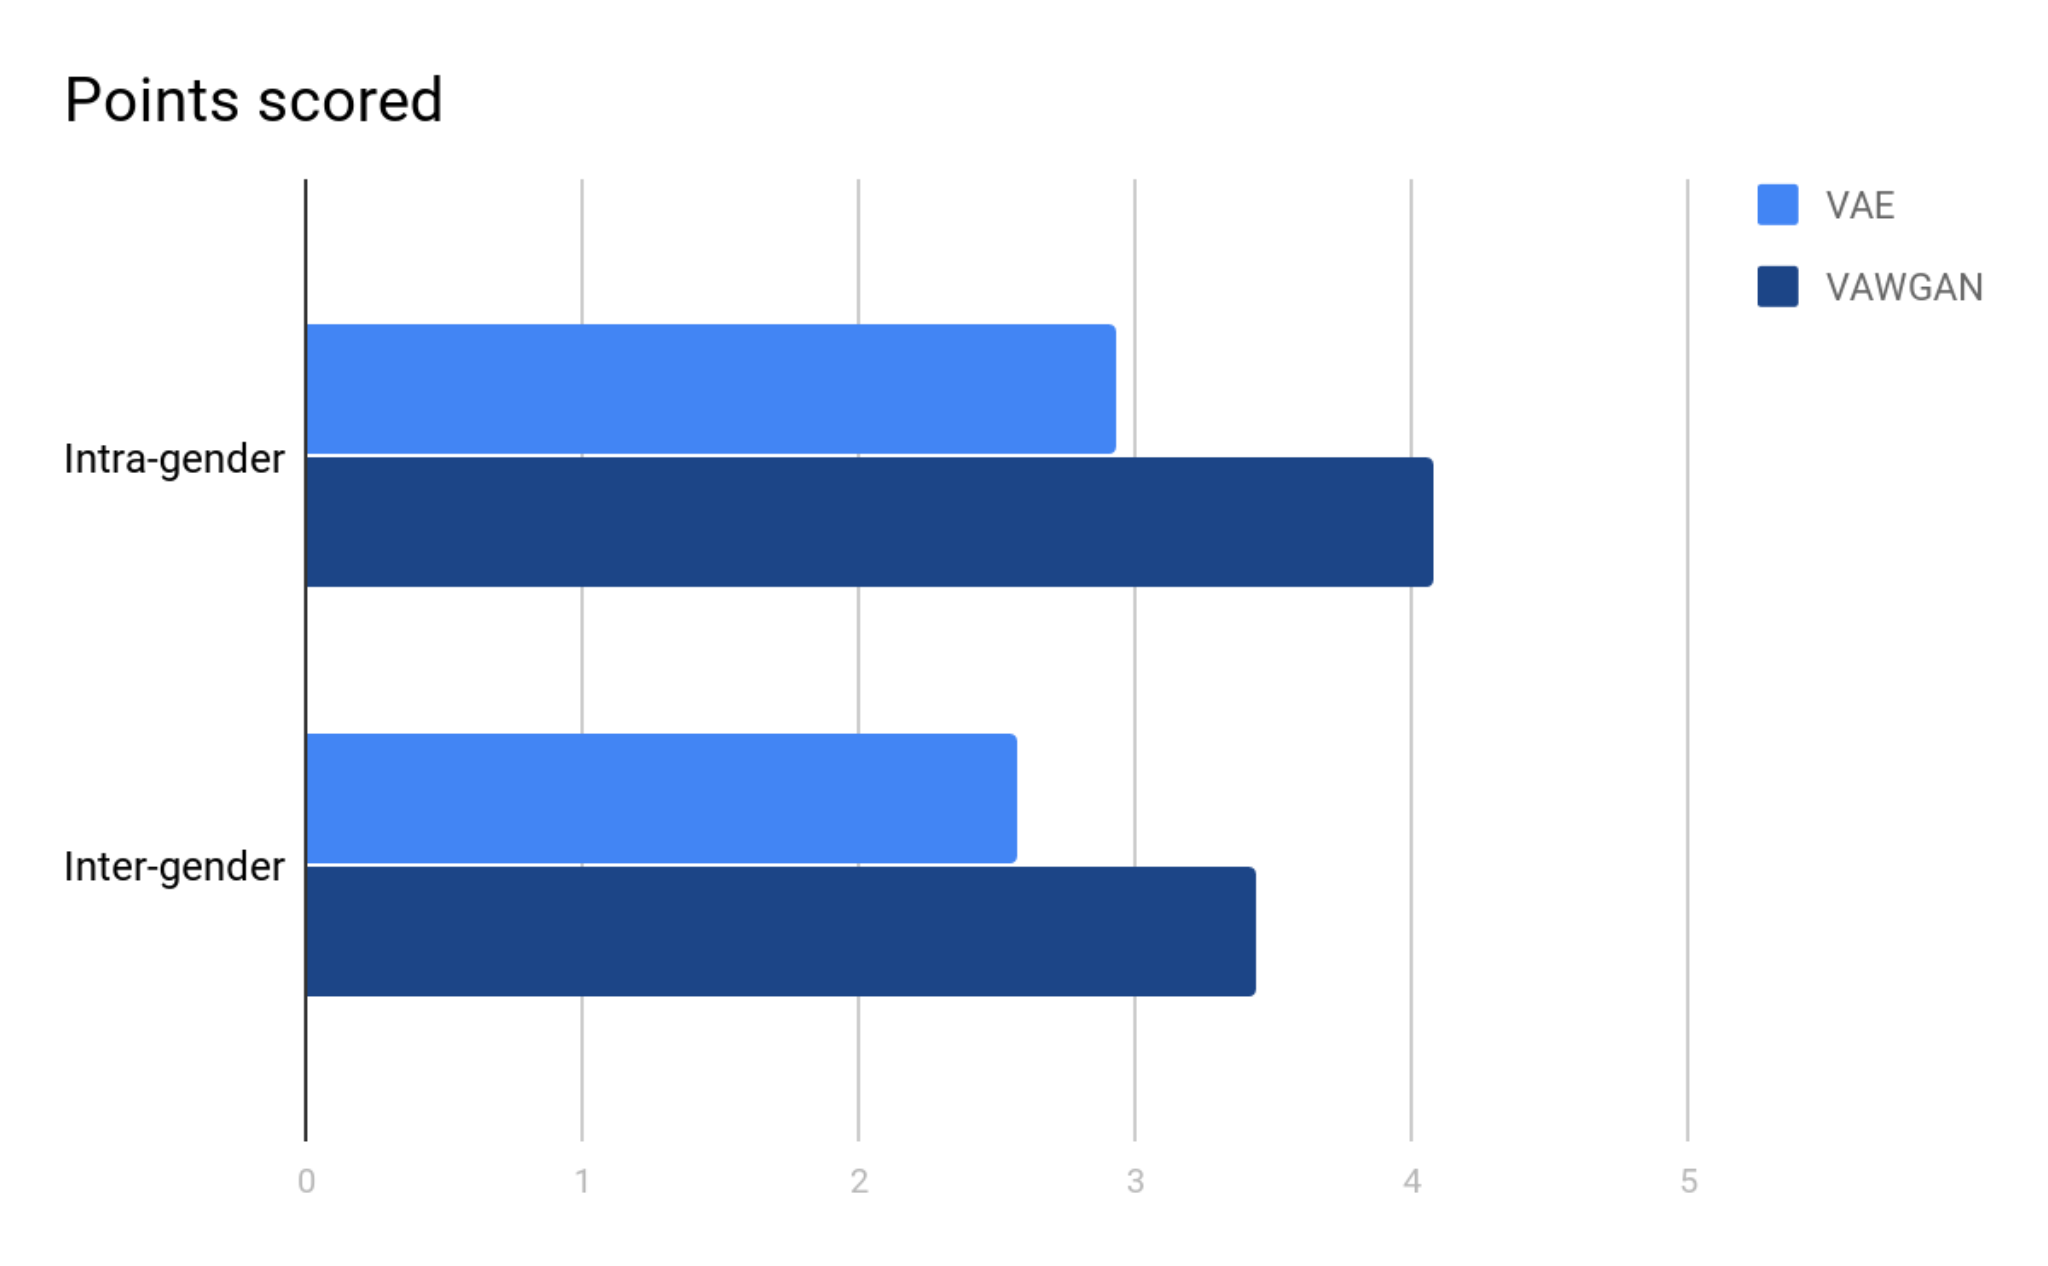
\includegraphics[width=8cm]{images/MOS}
    \caption{MOS for baseline and VAWGAN}
	\label{fig:mos}
\end{figure}

\begin{figure}[h]
	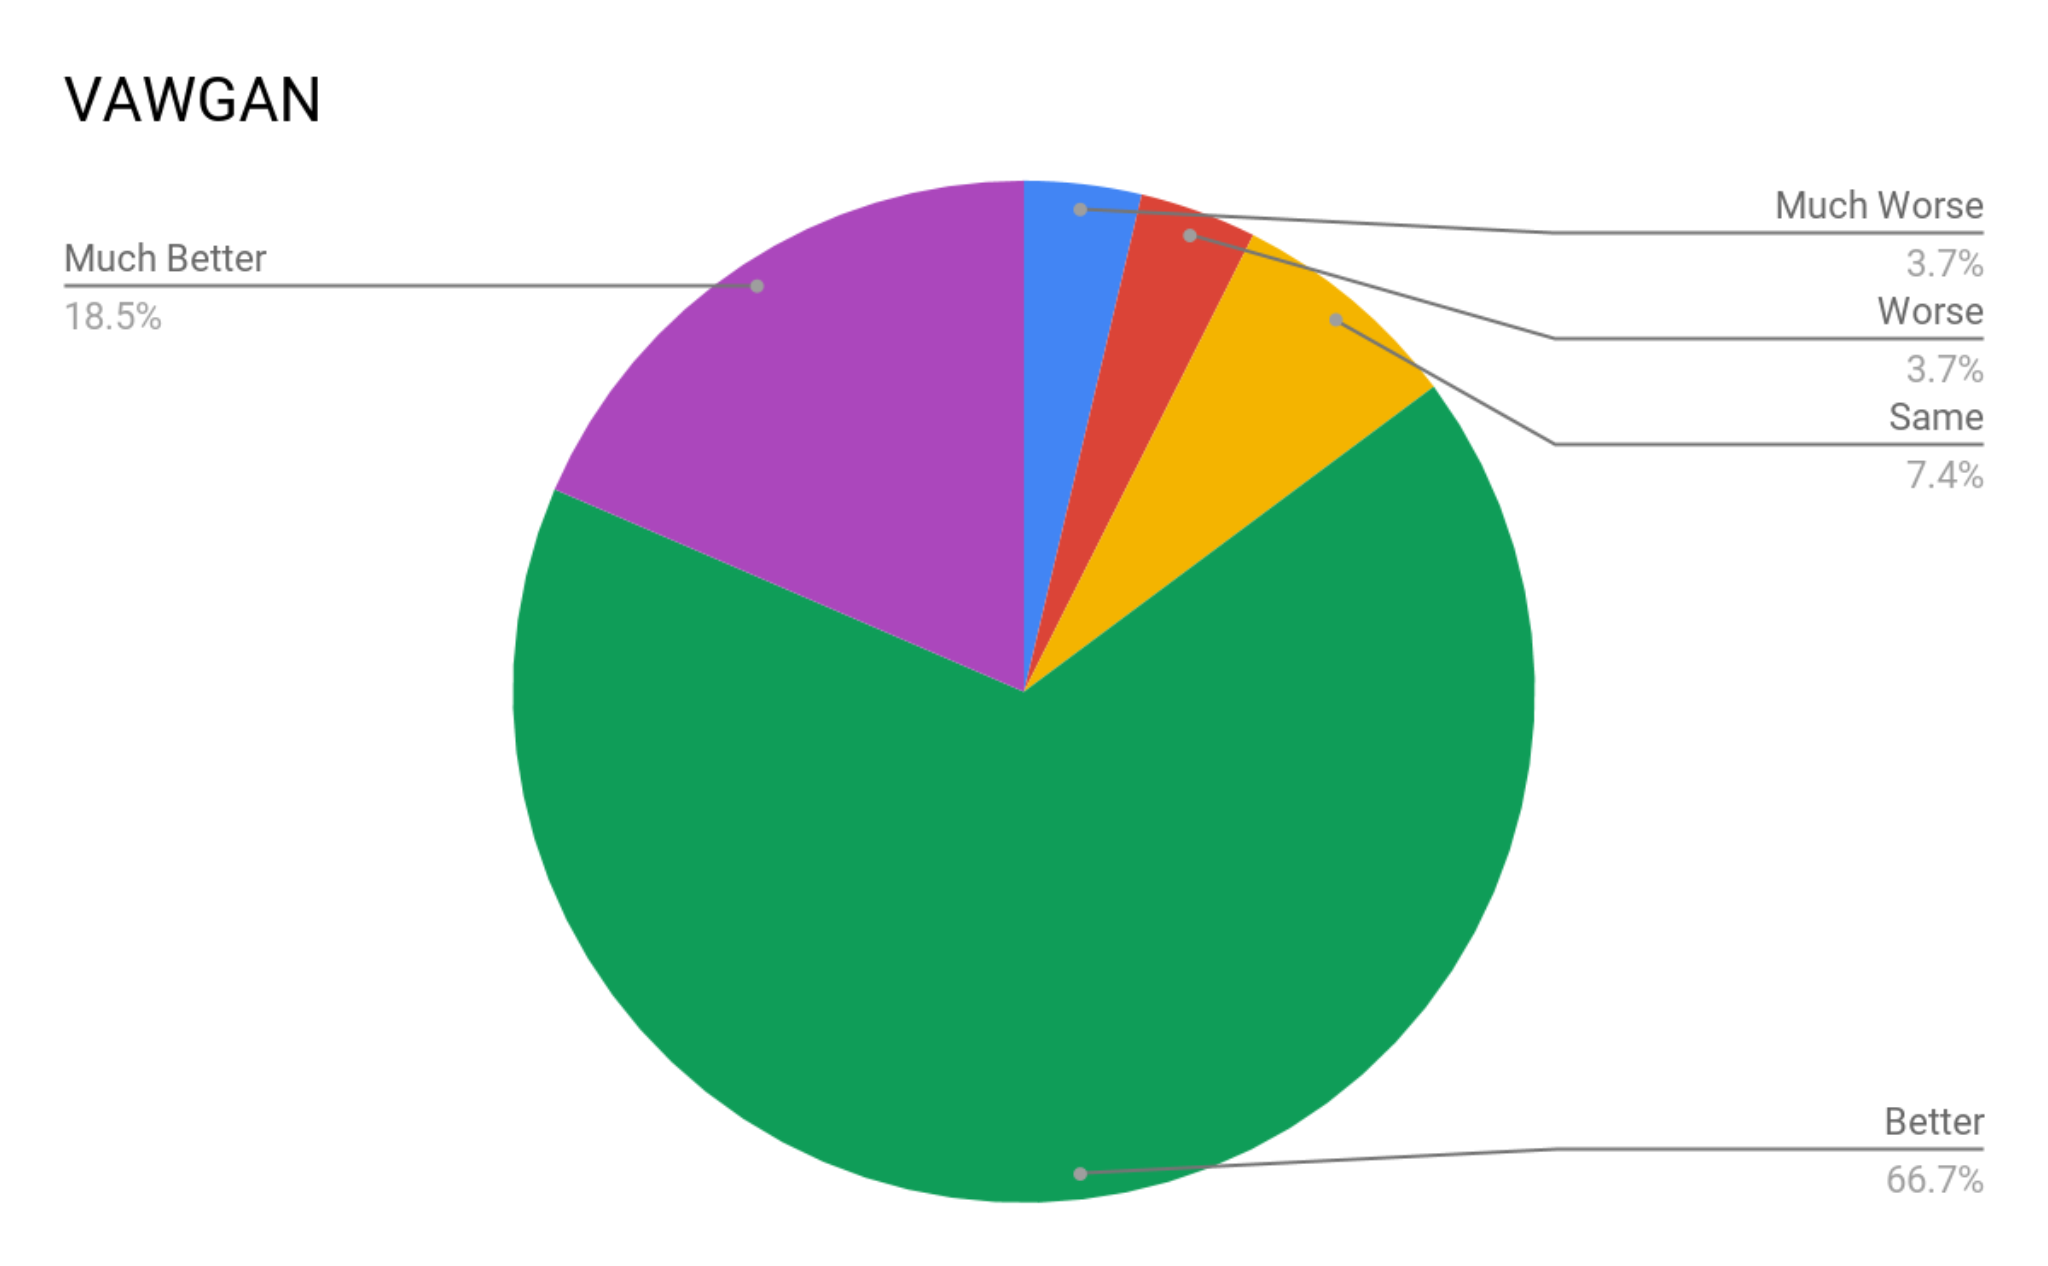
\includegraphics[width=8cm]{images/VAWGAN_versus_VAE}
    \caption{Qualitative comparison between baseline and VAWGAN}
	\label{fig:comparison}
\end{figure}

\begin{figure}[h]
	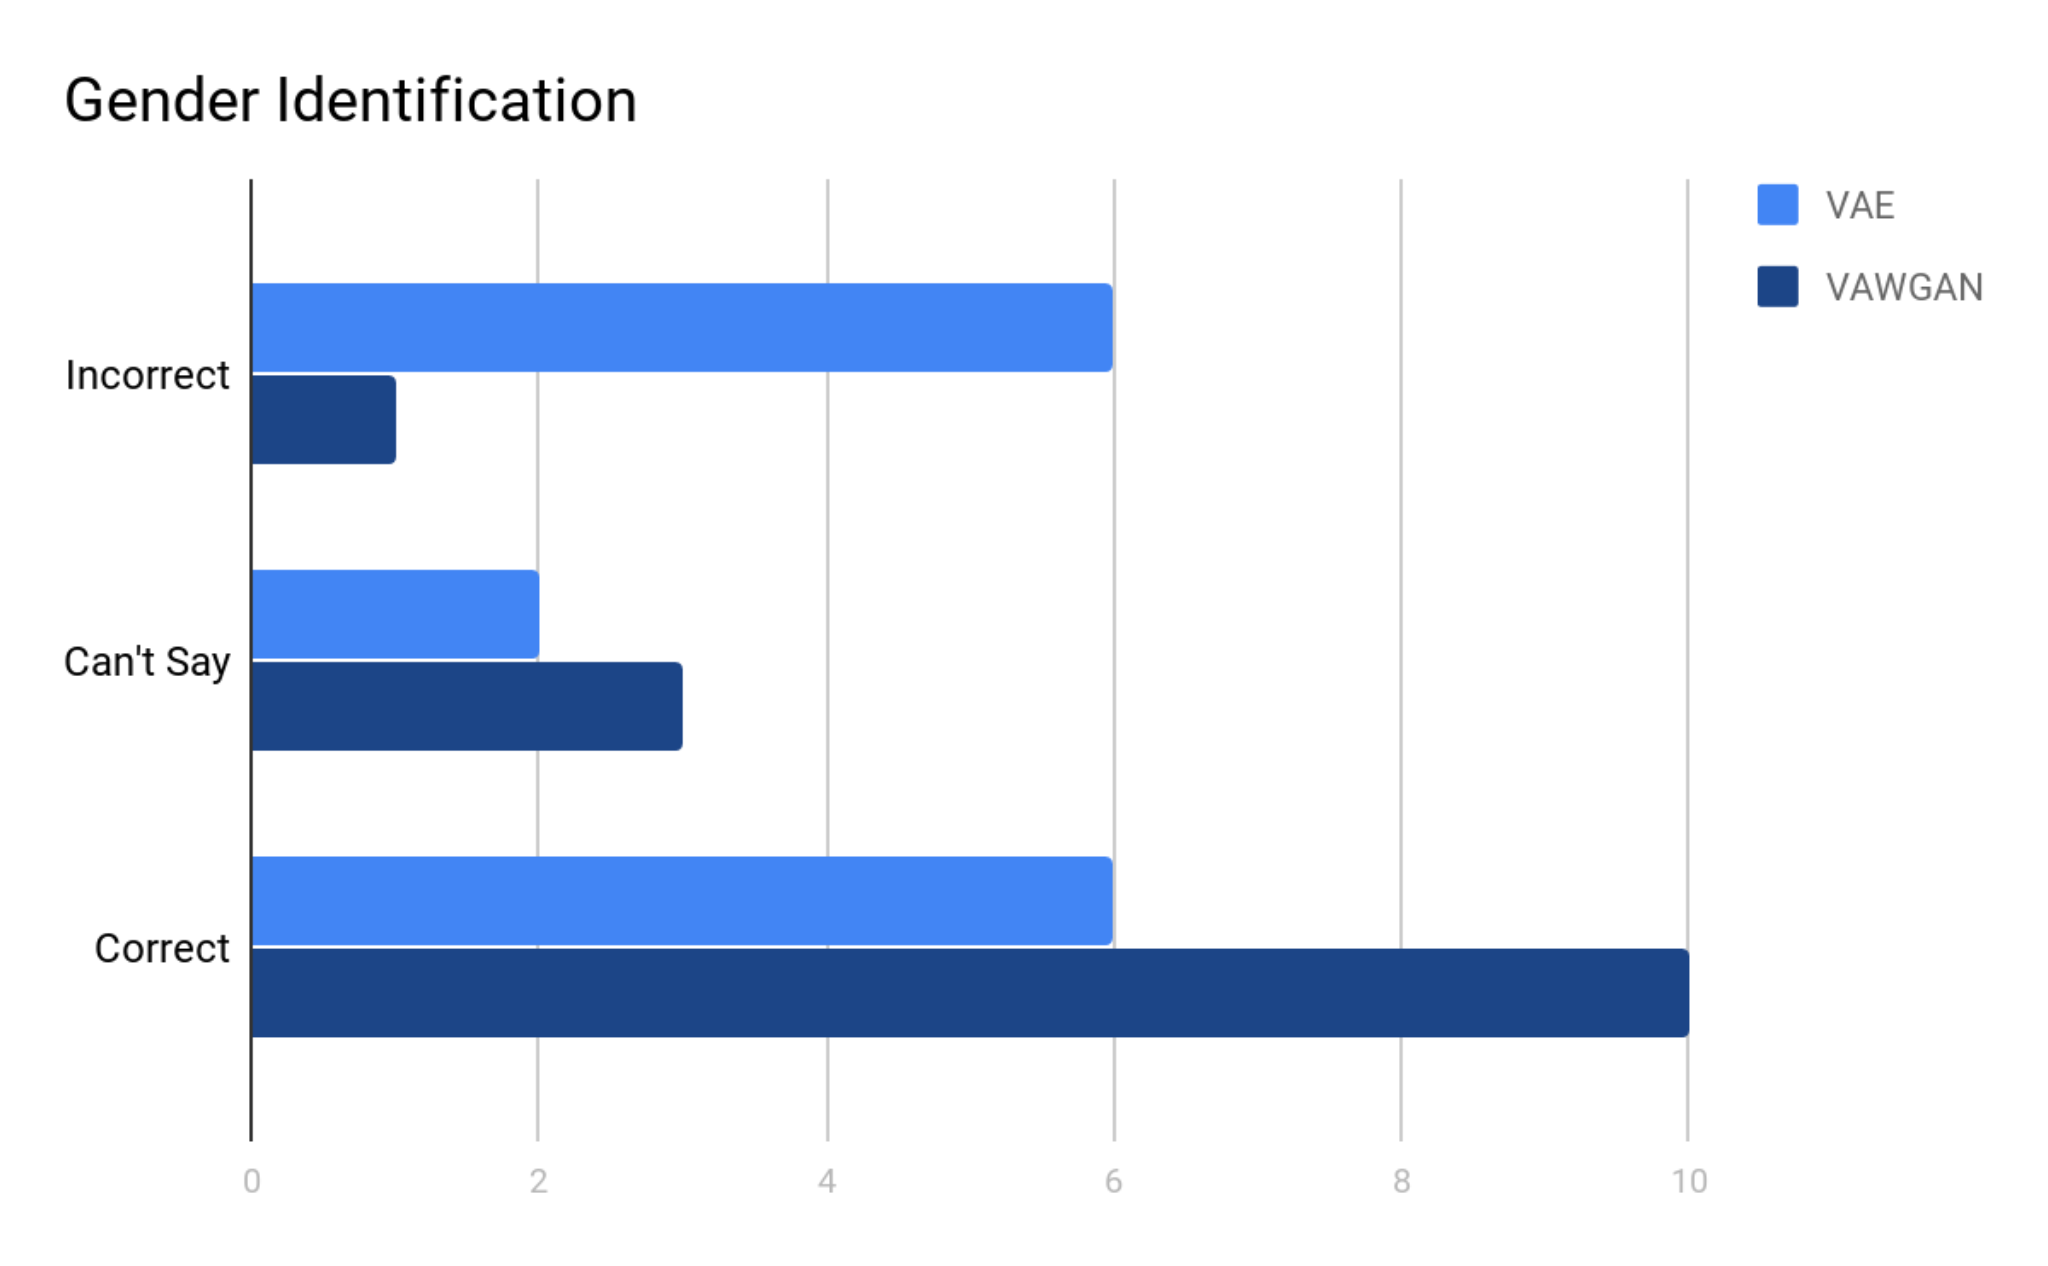
\includegraphics[width=8cm]{images/Gender_Identification}
    \caption{Gender Identification Results for baseline and VAWGAN}
	\label{fig:gender}
\end{figure}

\subsection{Future Work}

The quality of the audio generated is still not on par with the audio generated by parallel conversion and doesn't sound very natural. Since there is no alignment in the data, a non-parallel conversion relies on getting a good representation of the content and speaker which is used to generated converted voice.

The content representation is currently done with the help of an encoder. Instead, the word or phone sequence of the source speech can be generated using a automatic speech recognition system and used as the content representation. Our work on sentence embedding is a step in that direction.

Speaker representation is given in the form of a one-hot vector in this project. If better representation like i-vectors are given, the generator can use it for generating better conversions. Passing the speaker representation to the encoder might also help it encode only the speaker independent part, hence, improving the quality of content representation.

\section{Summary}

The results of voice conversion using VAE and WGAN given in \cite{vawgan} have been replicated. A novel method of extending it by using sentence embeddings as a representation of content has been developed.

In future, better speaker representation like i-vectors and better content representation can be used for improving encoding and generation.

\bibliographystyle{named}
\bibliography{ref}

\end{document}